\documentclass[tikz,border=6pt]{standalone}
\usepackage[T1]{fontenc}
\usepackage{lmodern}
\usetikzlibrary{arrows.meta,positioning,decorations.pathreplacing}
\definecolor{hc}{HTML}{2B4FA3}
\definecolor{ac}{HTML}{D7263D}
\definecolor{dc}{HTML}{BCC3CC}
\definecolor{ink}{HTML}{1F2933}
\begin{document}
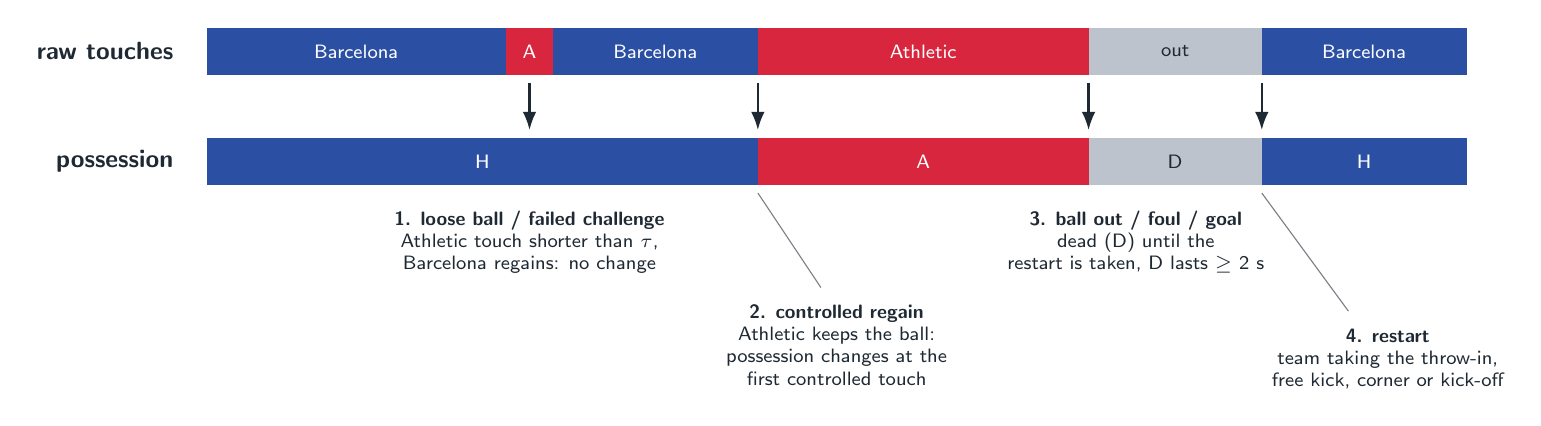
\begin{tikzpicture}[font=\sffamily\small, x=1mm, y=1mm,
  seg/.style={minimum height=7mm, inner sep=0pt, text=white, font=\sffamily\scriptsize\bfseries},
  note/.style={font=\sffamily\scriptsize, text=ink, align=center}]

% raw events row
\node[anchor=east, note, font=\sffamily\small\bfseries] at (-3,10) {raw touches};
\fill[hc] (0,7) rectangle (38,13);
\fill[ac] (38,7) rectangle (44,13);
\fill[hc] (44,7) rectangle (70,13);
\fill[ac] (70,7) rectangle (112,13);
\fill[dc] (112,7) rectangle (134,13);
\fill[hc] (134,7) rectangle (160,13);
\node[note, text=white] at (19,10) {Barcelona};
\node[note, text=white] at (41,10) {\scriptsize A};
\node[note, text=white] at (57,10) {Barcelona};
\node[note, text=white] at (91,10) {Athletic};
\node[note] at (123,10) {out};
\node[note, text=white] at (147,10) {Barcelona};

% possession row
\node[anchor=east, note, font=\sffamily\small\bfseries] at (-3,-4) {possession};
\fill[hc] (0,-7) rectangle (70,-1);
\fill[ac] (70,-7) rectangle (112,-1);
\fill[dc] (112,-7) rectangle (134,-1);
\fill[hc] (134,-7) rectangle (160,-1);
\node[note, text=white] at (35,-4) {H};
\node[note, text=white] at (91,-4) {A};
\node[note] at (123,-4) {D};
\node[note, text=white] at (147,-4) {H};

% annotations
\draw[-{Latex}, ink, thick] (41,6) -- (41,0);
\node[note, anchor=north] at (41,-9) {\textbf{1. loose ball / failed challenge}\\Athletic touch shorter than $\tau$,\\Barcelona regains: no change};
\draw[-{Latex}, ink, thick] (70,6) -- (70,0);
\node[note, anchor=north] at (80,-21) {\textbf{2. controlled regain}\\Athletic keeps the ball:\\possession changes at the\\first controlled touch};
\draw[ink!60] (70,-8) -- (78,-20);
\draw[-{Latex}, ink, thick] (112,6) -- (112,0);
\node[note, anchor=north] at (118,-9) {\textbf{3. ball out / foul / goal}\\dead (D) until the\\restart is taken, D lasts $\geq$ 2 s};
\draw[-{Latex}, ink, thick] (134,6) -- (134,0);
\node[note, anchor=north] at (150,-24) {\textbf{4. restart}\\team taking the throw-in,\\free kick, corner or kick-off};
\draw[ink!60] (134,-8) -- (145,-23);
\end{tikzpicture}
\end{document}
